% !TEX root = ../master.tex
\chapter{Implementation}
\label{chap:impl}

The previous chapter yielded a general execution plan that shall implemented in the coming 
section while utilizing the cluster computer at the \ac{DHBW}. 
For each implementation detail the specifically chosen values are given during the process. Each of the steps holds 
the possibilities for errors which will also be evaluated.
The outcome of the taken steps is only a partially functional Hadoop cluster.
The reasons and implications for this restricted outcome are given.
Suggestions for future projects how better results might be achieved is given in the end.

\section{Infrastructure Set-Up in OpenStack}

The foundation for the cluster architecture that has been illustrated in figure \vref{fig:architecture} are the host \acp{VM}, their storage and the network that connects them.
In the course of this process some minor adaptions are made to the proposed architecture.
Especially the \texttt{hadoop-master-0} node now also runs the \ac{HDFS} Datanode and YARN Nodemanager service and therefore has a storage volume attached to it.


To set up the cluster the web interface of OpenStack can be used, which is accessible at
\urlinline{https://controller.c4.dhbw-mannheim.de/} from within the \ac{DHBW} network.
Each operation on the infrastructure can be performed within this interface.

\subsection{Execution}

\subsubsection{Firewall Rules}

TODO sec group considerations, which ports in out? 
default: out is open, in is only ping and ssh on 22
hadoop: detailed view \autocite[][]{hortonworks2017reference}, but for easier development temporary all ports incoming open. most important: 8080 for ambari


\subsubsection{Network}


\begin{figure}[hbt]
  {\centering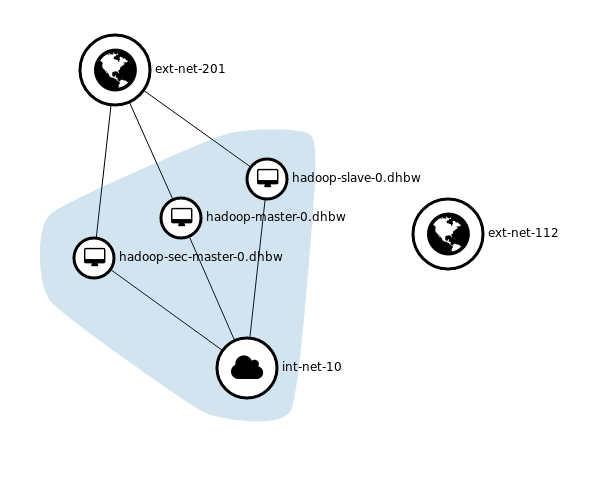
\includegraphics[width=0.8\textwidth]{{img/network_topology}.png}\par}
  \caption{Network topology created in OpenStack}
  \label{fig:network_topology}
\end{figure}

\begin{table}[hbt]
\resizebox{\textwidth}{!}{%
	\begin{tabular}{lll}
	  Network Name & Sub-networks & Descirption\\
	  \hline
	  ext-net-201 & 141.72.191.0/24 & Pre-existing connection to \ac{DHBW} internal network\\
	  ext-net-112 & 192.168.112.0/20 & Pre-existing connection with unknown destination\\
	  int-net-10 & 10.100.10.0/24 &  New internal network used by Hadoop\\
	\end{tabular}%
	}
	\caption{Sub-Networks with in the projekt in OpenStack}
	\label{fig:networks_subnets}
\end{table}

TODO new internal network chosen from private address space (defined in RFC~1918 by the the Internet Engineering Task Force \autocite[][]{ietf1996rfc1918})

\subsubsection{Virtual Machines}

TODO do the math on resources

\begin{table}[hbt]
\centering
\resizebox{0.8\textwidth}{!}{%
	\begin{tabular}{lrl}
	  Resource Type & Amount & Unit\\
	  \hline
	  Instances & 10 & \\
	  \acp{VCPU} & 20 & \\
	  \acs{RAM} & 51200 & \ac{MB} \\
	  Floating \ac{IP} Addresses & 10 & \\
	  Security Groups & 10 & \\
	  Volumes & 10 & \\
	  Volume Storage & 1000 & \ac{GB}
	\end{tabular}%
	}
	\caption{Available resources for the project in the \ac{DHBW} OpenStack environment}
	\label{fig:resources_openstack}
\end{table}

\begin{table}[hbt]
\centering
\resizebox{0.8\textwidth}{!}{%
	\begin{tabular}{lrrr}
	  Instance Flavor Name & \acp{VCPU} & \ac{RAM} & Root Disk Size \\
	  \hline
	  m1.nano & 1 & 64~\ac{MB} & 1~\ac{GB} \\
	  m1.tiny & 1 & 512~\ac{MB} & 5~\ac{GB} \\
	  m1.small & 1 & 1~\ac{GB} & 10~\ac{GB} \\
	  m1.medium & 2 & 2~\ac{GB} & 20~\ac{GB} \\
	  m1.large & 4 & 4~\ac{GB} & 40~\ac{GB} \\
	  m1.xlarge & 8 & 8~\ac{GB} & 80~\ac{GB} \\
	\end{tabular}%
	}
	\caption{Available instance sizes in the \ac{DHBW} OpenStack environment}
	\label{fig:instance_sizes}
\end{table}

\subsubsection{Storage}

TODO
create disks
assing them
format them
ansible will be used to mount them

\subsection{Encountered Issues and Lessons Learned}

TODO Access only from dhbw on site net leads to difficult development conditions where author needs to be on site and is restricted by the locality

TODO Network connection unstable leading to more difficult environment with regular loss of connectivity to server

TODO Internal errors within openstack (temporary) where not enough resources could be allocated to get the requested VMs, later resolved


\section{System Set-Up with Ansible}

\subsection{Preparation}

\subsection{Execution}

\subsection{Encountered Issues and Lessons Learned}

TODO as expected the larger root partition of 80 GB was enough for the selected services

TODO memory on master node was exceeded even with not all services runnig (only)


\section{Hadoop Set-Up with Ambari}

\subsection{Preparation}

TODO explain and maybe print this particular playbook yes yes print it with explainations

\subsection{Execution}

\subsection{Encountered Issues and Lessons Learned}

\section{System Tests}

\section{Conclusion}

TODO dhbw cloud is unreliable af

TODO process is way too hard for and too long for students to do in a lecture without depper understanding of sysadmin  

Abweichen von architecture war dumm, da memory knapp durch zu viele prozesse



TODO HELP ME IM STREGGELING WITH EXISTENCE

\urlinline{https://docs.hortonworks.com/HDPDocuments/Ambari-2.6.1.5/bk_ambari-installation/bk_ambari-installation.pdf}


TODO ref exec plan

TODO Tools will be Apache Spark, Storm, Hive und Pig

TODO openstack

    ATTENTION: Network connection: sometimes due to a bug in openstack first only outer network connection then attach inner connection and reboot at least in bwclound, in dhbw works. 
    , note down the eth port that is newly created for internal connection.
    


TODO Ansible
see \urlinline{https://github.com/XOSplicer/studienarbeit-hadoop-cluster-ansible}
     (in implementation explain how the ansible part works). 
     
     should create also new user which is allowed to be accessed via SSH and  password so that hadoop can be used from this account

TODO Ambari

    TODO ,  when promted to select nodes use manual registaration: reason dont upload ssh private key for root access (maybe in chpt 4).

TODO Tests

HDFS WORKS
YARN is broken
mapred is broken

\urlinline{https://gist.github.com/ace-subido/0a9b219b2348921f6a87/3141000d2cbb0f78b967b75304908f4289aa8f01}

\urlinline{https://www.ripublication.com/ijaer18/ijaerv13n6_166.pdf}
\urlinline{http://sortbenchmark.org/YahooHadoop.pdf}
\urlinline{http://citeseerx.ist.psu.edu/viewdoc/download?doi=10.1.1.178.1187&rep=rep1&type=pdf}

\urlinline{https://hadoop.apache.org/docs/r1.0.4/api/org/apache/hadoop/examples/terasort/TeraGen.html}\\urlinline{https://www.systutorials.com/3235/hadoop-terasort-benchmark/} (also mentioned in \autocite[][]{white2015hadoop})


\urlinline{https://www.cloudera.com/documentation/enterprise/latest/topics/cdh_ig_ports_cdh5.html}

TODO

TODO maintainability
